\chapter{The GERDA experiment}
\label{cha:gerda}
The GERDA (GERmanium Detector Array) experiment \cite{Abt04, Sch05} is
designed to search for the $0\nu\beta\beta$ decay of $^{76}$Ge. The
physics reach will depend on the achievable background level. The main
design feature is to operate ``naked'' germanium detectors directly in
liquid argon in order to make an extremely low background level
possible. The concept is based on ideas presented in
Ref.~\cite{Heu95}. The experiment is described in the first section of
this chapter. GERDA is currently under construction in Hall A of the
INFN Gran Sasso National Laboratory (LNGS), Italy. The current status
of the experiment is given in the second section. GERDA is planned in
three phases. In the first phase (Phase I) unsegmented germanium
detectors, which were previously used in the IGEX \cite{Aal02} and HdM
\cite{Hei04} experiments, will be re-deployed. The envisioned
background level is $10^{-2}$~events/(kg$\cdot$keV$\cdot$year). In the
second phase (Phase II), in addition, 18-fold segmented detectors will
be used. The background level aimed at is
$10^{-3}$~events/(kg$\cdot$keV$\cdot$year). A later phase (Phase III)
is under discussion in cooperation with the Majorana collaboration
\cite{Gai03, Aal04}, aiming at a one-ton experiment. The physics
observation capability of GERDA is discussed in the last section.

\section{Background reduction techniques}
\label{sec:gerda:conc}
Germanium detectors have been used to detect ionizing radiation,
particularly X-rays and $\gamma$-rays, for decades. The energy
resolution is typically better than 1\% around the $Q$-value of the
$^{76}$Ge $\beta\beta$ decay. This is among the best of all detectors
introduced in Sec.~\ref{sec:gencon} and provides a very good
separation between the $0\nu\beta\beta$ signal and the
$2\nu\beta\beta$ background. However, the natural abundance of
$^{76}$Ge is only 7.6\%. As both signal and background scale with
mass, isotopic enrichment is needed to improve the signal to
background ratio. In addition, the $Q$-value of the $0\nu\beta\beta$
decay of $^{76}$Ge, 2.039~MeV, is lower than some lines prominent in
natural radioactivity. Therefore the design of the experiment has to
minimize the amount of radioactive elements in the vicinity of the
detectors. Fig.~\ref{fig:gerda} is an artist's view of GERDA. Each
part of the experiment is introduced in the following sections and its
function in reducing background is discussed.

\begin{figure}[tbhp]
\centering
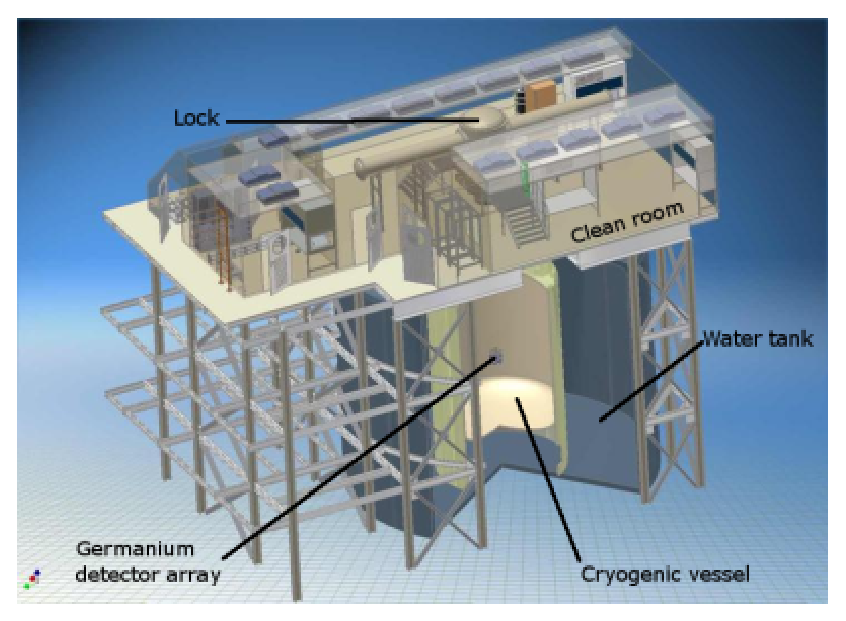
\includegraphics[width=0.7\textwidth]{gerda}
\caption{Artist view of GERDA. An array of germanium detectors is
submerged in liquid argon inside a cryogenic vessel surrounded by a
water tank. A lock system inside the clean room above the water tank
provides access to the cryogenic volume.}
\label{fig:gerda}
\end{figure}

\subsection{Underground location and muon veto}
\label{sec:gerda:loca}
To reduce the cosmic ray induced background GERDA is located
underground, in Hall A of the INFN\footnote{Istituto Nazionale di
Fisica Nucleare} Gran Sasso National Laboratory (LNGS), Italy. LNGS is
the largest underground facility in the world for low-background
experiments. It is accessed from the 10~km long highway tunnel under
the Gran Sasso mountains. It has three experimental halls hosting a
large variety of experiments, most of which focus on dark matter or
neutrino physics. Fig.~\ref{fig:lngs} shows the location of GERDA
inside LNGS. The main experimental site of GERDA is between the Large
Volume Detector (LVD) and the service tunnel crossing Hall A. The
GERDA auxiliary and cryogenic storage system will be located in the
service tunnel on the northeast side of Hall A.

\begin{figure}[tbhp]
\centering
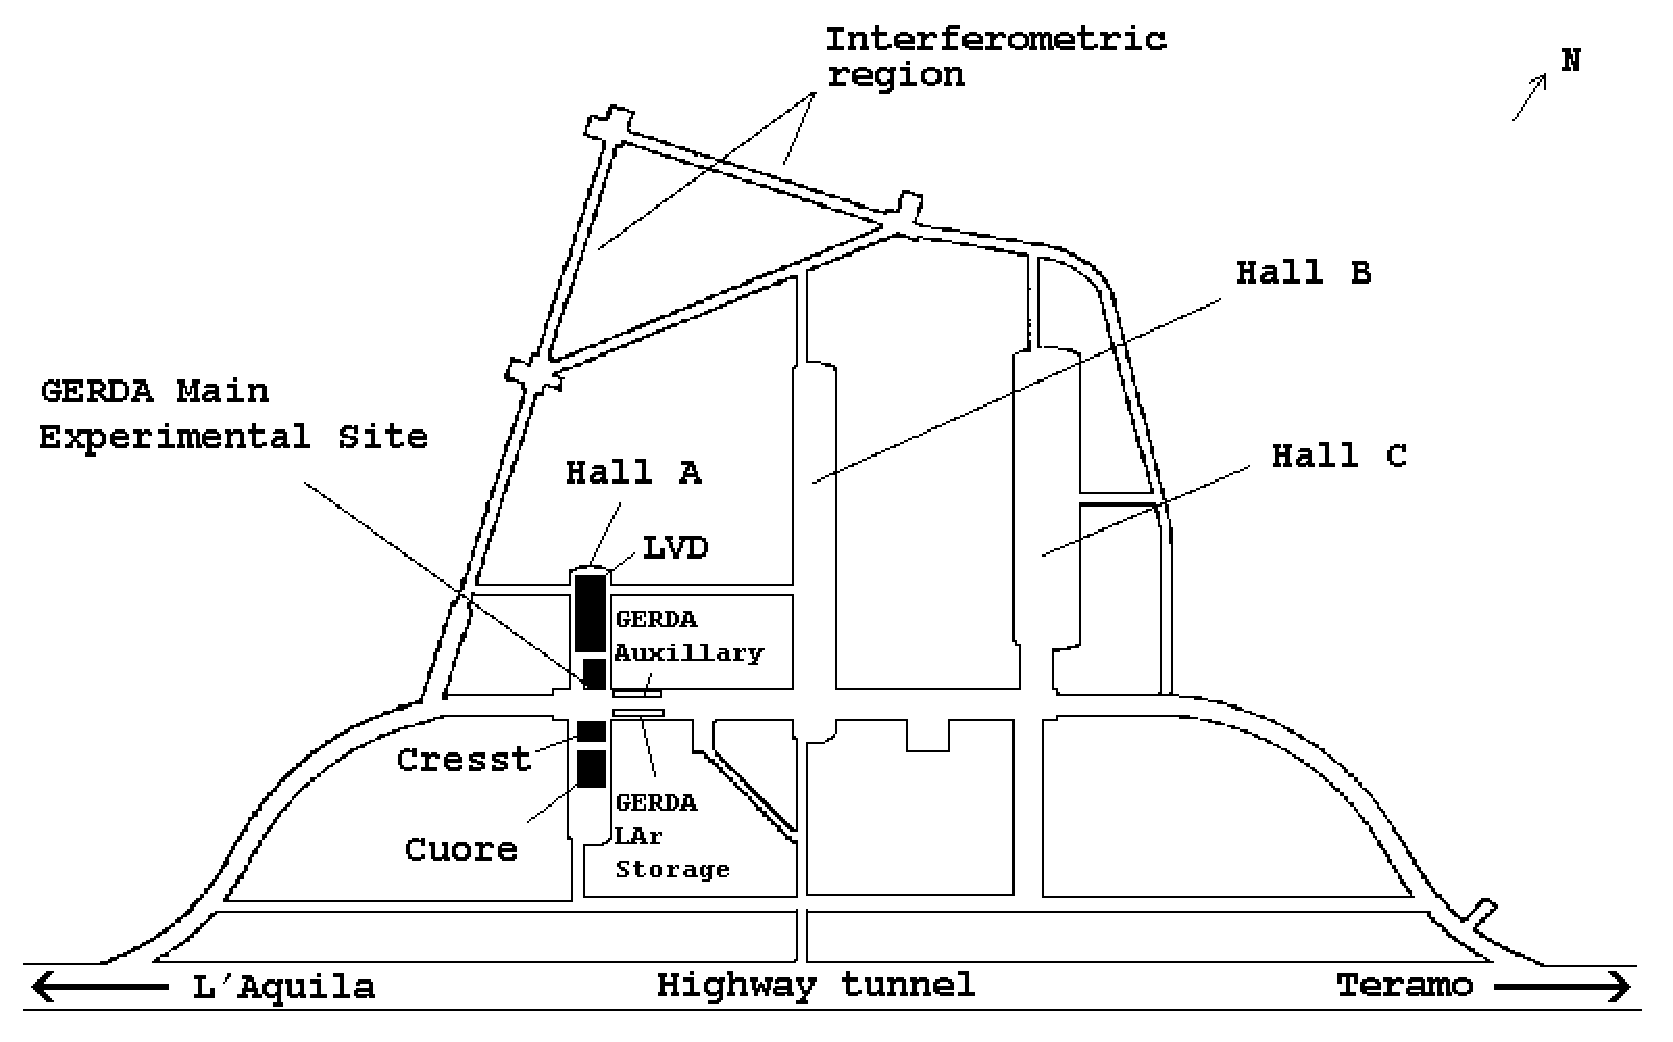
\includegraphics[width=0.8\textwidth]{lngs}  
\caption{Location of GERDA inside LNGS. The main experimental site of
GERDA is between the Large Volume Detector (LVD) and a service tunnel
crossing Hall A. The GERDA auxiliary and cryogenic storage system will
be located in the service tunnel on the northeast side of Hall A.}
\label{fig:lngs}
\end{figure}

The overburden of 1.4~km of rock above the experimental halls
corresponds to 3400 meter of water equivalent (m.w.e). It reduces the
cosmic ray induced muon (neutron) flux by a factor of $10^{6}$
($10^{3}$) compared to the surface. The energy and angular
distributions of cosmic ray muons in Hall A of LNGS have been
precisely measured \cite{Amb95, Lip91, Amb03}. A comprehensive study
of cosmic ray induced muon and neutron background in underground
laboratories can be found in Ref.~\cite{Mei06}.

In order to further reduce the muon induced background an additional
muon veto system will be installed. Cosmic muons traversing the water
tank (see Fig.~\ref{fig:gerda}) will cause \u{C}erenkov radiation. To
detect the radiation 66 photomultiplier tubes (PMTs) will be installed
on the walls of the water tank. The positions of the PMTs are
optimized according to Monte Carlo simulation. The detection
efficiency is about 95\% depending on the incident angle of the
muon. In order to compensate for the missing water around the neck of
the cryostat plastic scintillator plates will be placed on top of the
clean room. They will be used to detect the muons entering the
cryostat almost vertically. The combined detection efficiency is
expected to be above 99\%.

\subsection{Water tank and cryostat}
\label{sec:gerda:rock}
To shield against neutron radiation from the surrounding rock about
630~m$^{3}$ of ultra-pure water will be filled in a stainless steel
tank with an outer diameter of 10~m and a height of about 8~m. The
stainless steel cryostat inside the water tank has an internal copper
lining. The height of the vessel is 5.88~m (7.62~m with the neck) with
an outer diameter of 4.16~m. It can contain 98~t of liquid argon. As
liquid argon can be produced with a much greater purity than lead or
even copper traditionally used for shielding, this minimizes the
radioactivity close to the detector array. The liquid argon also acts
as a shield against $\gamma$-rays, especially originating from the
cryostat itself.

\subsection{Detector array and electronics}
\label{sec:gerda:cable}
The germanium detectors will be lowered into the liquid argon from the
top of the cryostat. In order to minimize the radioactivity from the
suspension system low mass detector holders and minimal cabling will
be used (See Fig.~\ref{fig:holder1} and \ref{fig:holder2}). The
holders are made out of thin ultra-pure copper with a total weight of
about 30~g per detector. They are chained together vertically into
strings. Each string consists of up to five (most likely three)
detectors of the same type as shown in Fig.~\ref{fig:array2}. The
whole detector array could maximally consists of 16 hexagonally packed
detector strings as shown in Fig.~\ref{fig:atop}.

The horizontal distance between the centers of two detectors is
9~cm. The vertical clearance between two detectors is about 6~cm. The
Phase I detectors are p-type diodes with a cylindrical closed-ended
coaxial geometry. The detectors are enriched in $^{76}$Ge to a level
of about 86\% and have masses between 0.9~kg and 2.9~kg. Two options
are under consideration for GERDA Phase II. The norminal configuration
consists of 18-fold segmented $n$-type detectors. A second solution
based on point-contact $p$-type detecters is also under
consideration. In this thesis, we focus on the normial solution. The
precise size of the detectors in this solution will depend on
manufacturing details. The most likely dimensions are a height of
70~mm and a diameter of 75~mm. The detectors will be segmented 6-fold
in the azimuthal angle $\phi$ and a 3-fold in the height z.

\begin{figure}[tbhp]
\centering
\subfloat[]{\label{fig:holder1}
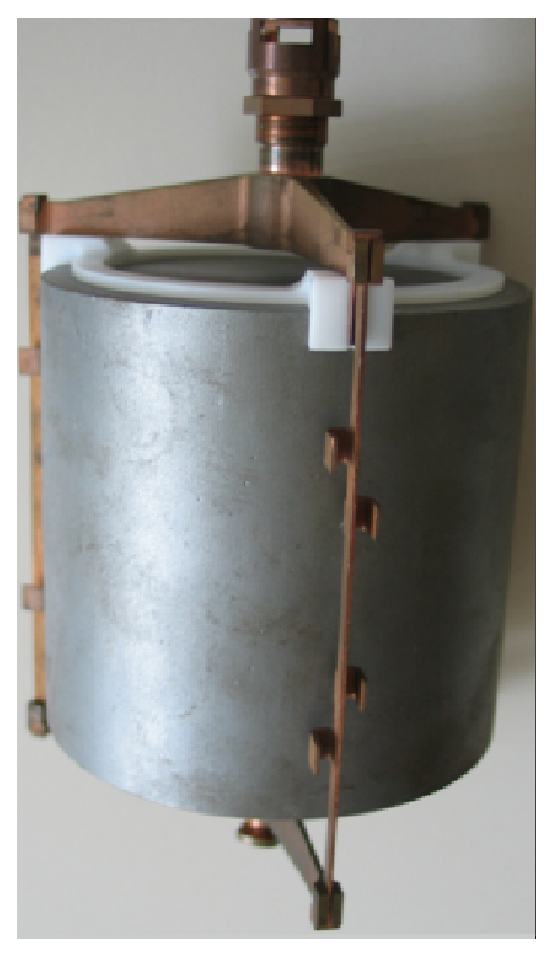
\includegraphics[height=0.23\textheight]{detectorHolderI}}\hfil %
\subfloat[]{\label{fig:holder2}
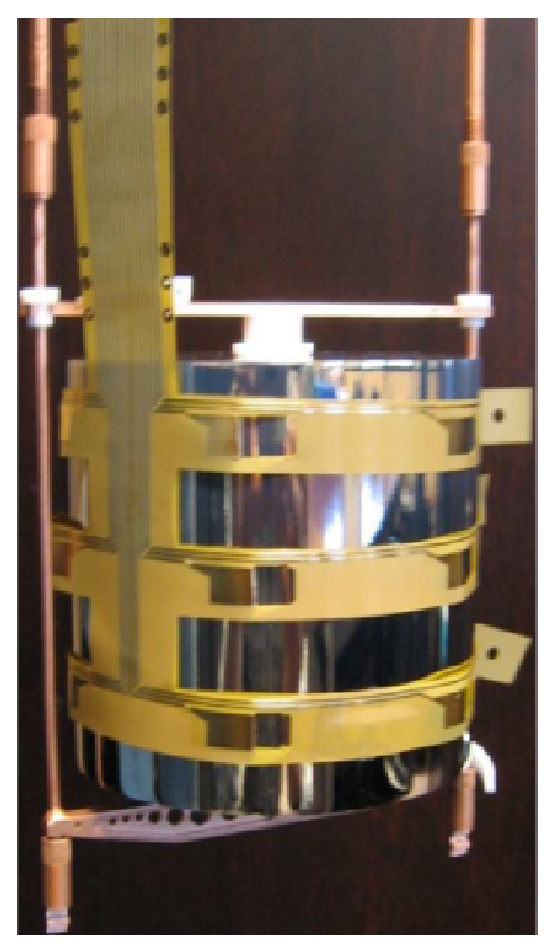
\includegraphics[height=0.23\textheight]{detectorHolderII}}\hfil%
\subfloat[]{\label{fig:array2}
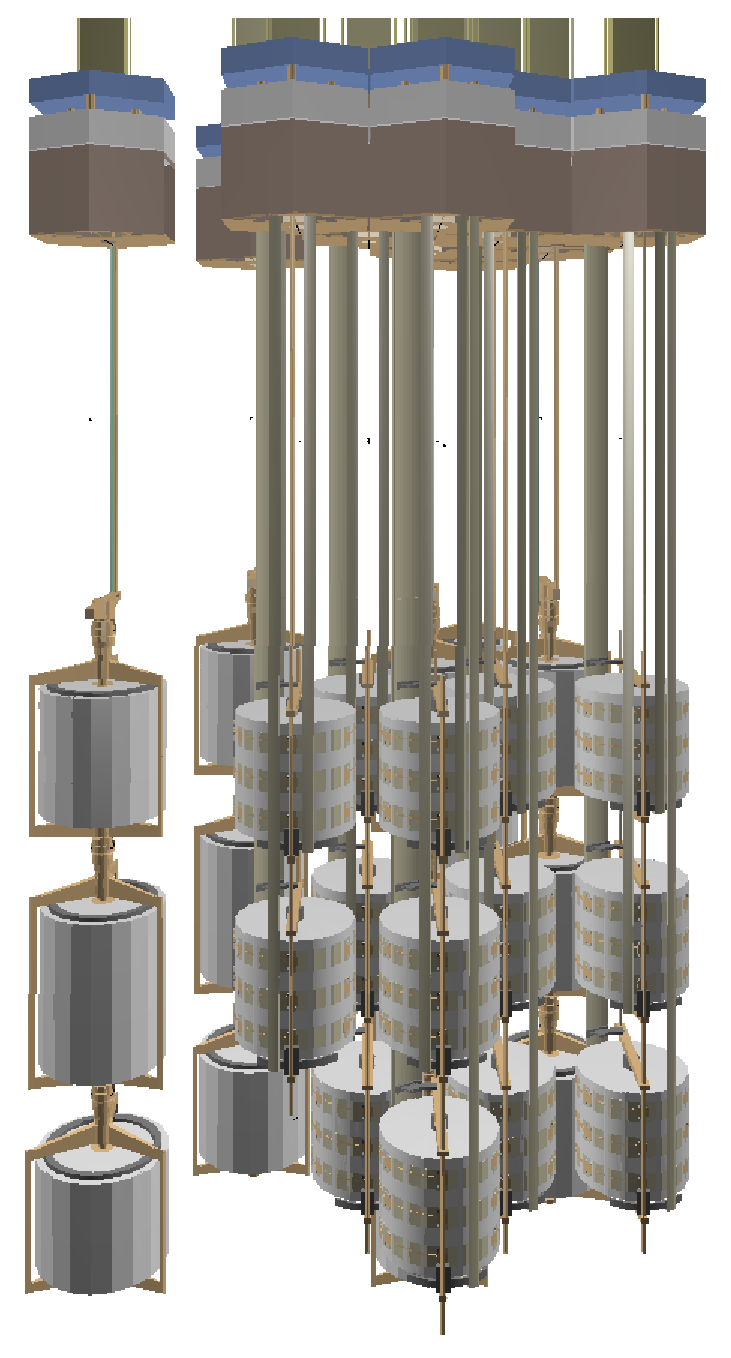
\includegraphics[height=0.23\textheight]{array}}%
\subfloat[]{\label{fig:atop}
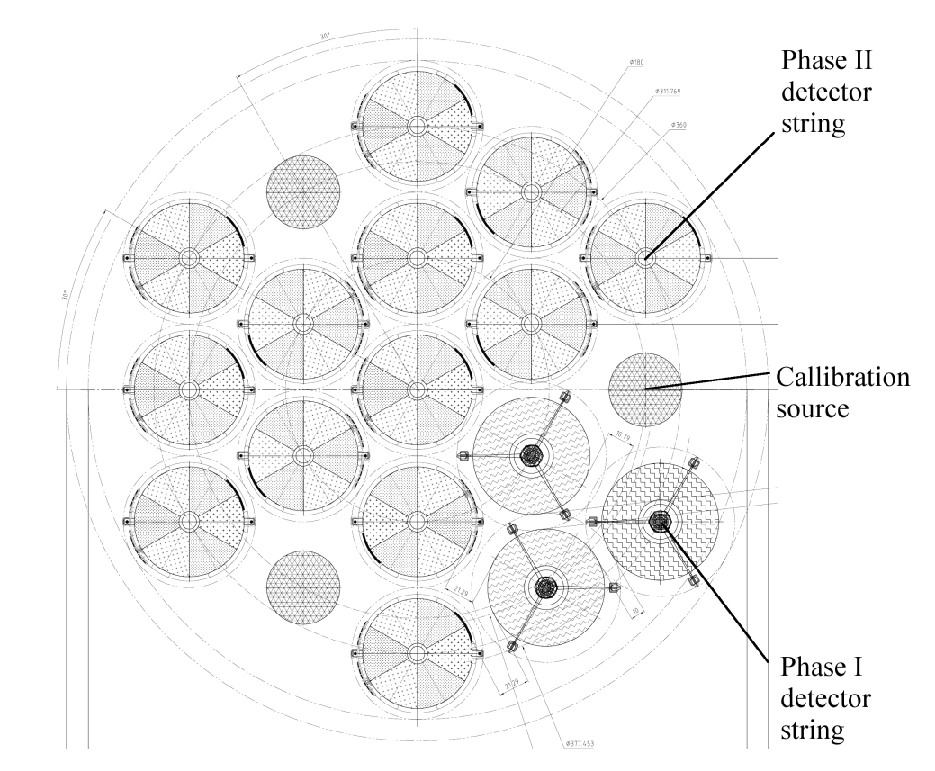
\includegraphics[height=0.23\textheight]{arrayTop}}%
\caption{Detector array configuration: (a) a single Phase I detector
in its copper holder, (b) a single Phase II detector in its copper
frame and with contact cable, (c) Phase II detector array and (d) top
view of the full array indicating the possible positions for Phase I
and Phase II detector strings as well as for the calibration sources.}
\label{fig:array}
\end{figure}

A couple of solutions are actively pursued for the read-out
electronics of GERDA \cite{Cat07}. A likely scheme foresees a cold FET
close to the crystal followed by amplifying and load driving circuits
located at room temperature. The cold FET would be placed near the
connection matrix (top blocks in Fig.~\ref{fig:array2}), 30~cm above
the detector array. Pre-amplified signals would be sent to electronics
located outside the lock system at room temperature through at least
6~m long cables.

\subsection{Detector storage and clean room}
\label{sec:gerda:source}
Whenever above ground, germanium detectors are exposed to cosmic
radiation and radioactive isotopes are produced inside the detector
through spallation caused by energetic cosmic rays. Two cosmogenic
isotopes, $^{60}$Co and $^{68}$Ge, have Q-values above that of
$^{76}$Ge $0\nu\beta\beta$ decay and are potential sources of
background. Therefore the time above ground needs to be
minimized. Since the half life time of $^{60}$Co and $^{68}$Ge is 5.3
years and 271 days, respectively, a passive method to reduce the
contamination is to keep the detectors long enough underground and
wait for it to decay.

When exposed to air the surface a germanium detector can collect dust
which contains many radioactive isotopes, particularly Pb$^{214}$,
undergoing $\alpha$ decay. Some parts of the detector surface are not
fully charge sensitive and only part of the energy lost by the
$\alpha$ particle can be detected. This may result in a signal close
to the $Q$-value of the $^{76}$Ge $0\nu\beta\beta$ decay. Therefore
the testing, preparation and insertion of the detector has to be done
in a clean environment. For this purpose, a class 10000 clean room
with radon-reduced air will be built on top of the cryostat. It houses
a lock, through which detector strings are inserted into and removed
from the cryogenic volume. Detector handling will be performed in
flow-boxes and a detector mounting-station which will reach class 100.
The lock consists of a rail system which allows to move detector
strings into their correct position and lower them into the
cryostat. In addition, the clean room will be used to temporarily
store germanium detectors in a controlled atmosphere of gaseous argon
or vacuum as shown in Fig.~\ref{fig:store}.

\begin{figure}[tbhp]
\centering
\subfloat[]{\label{fig:ounit}
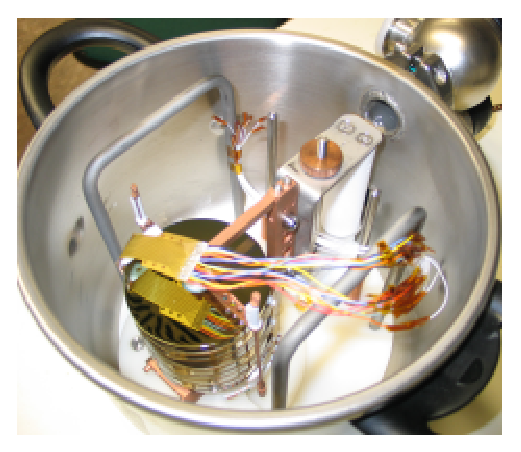
\includegraphics[height=0.1\textheight]{openUnit}}%
\subfloat[]{\label{fig:cunit}
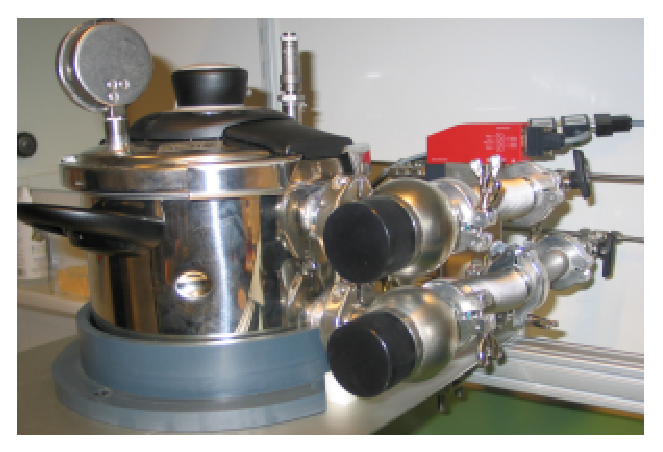
\includegraphics[height=0.1\textheight]{closedUnit}}%
\subfloat[]{\label{fig:sunit}
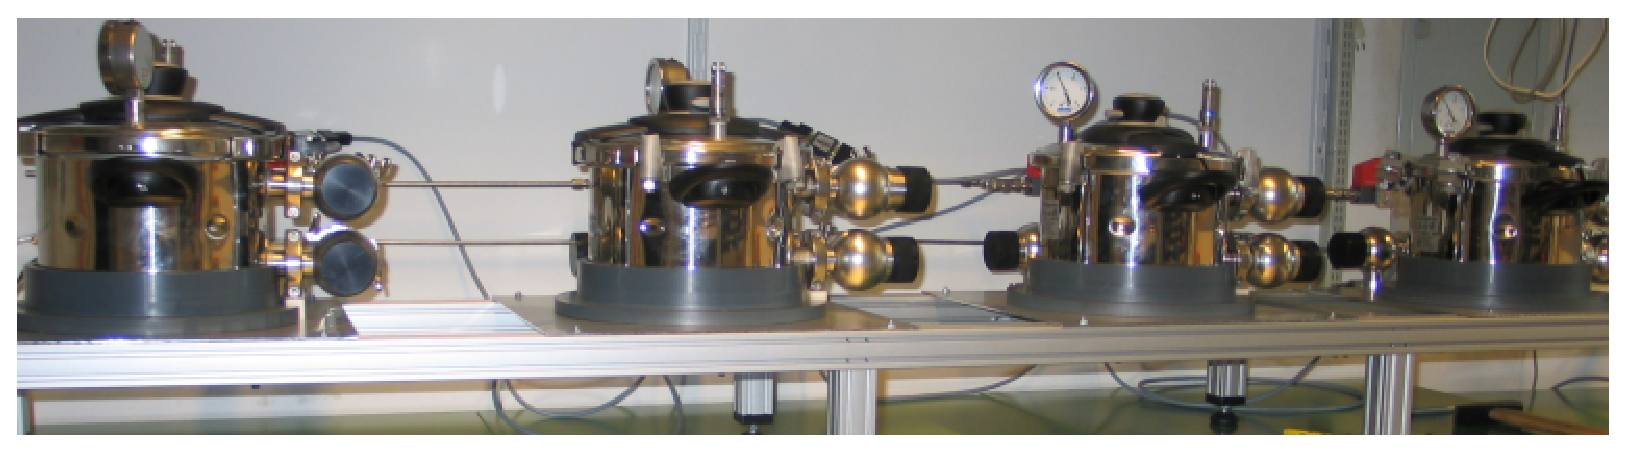
\includegraphics[height=0.1\textheight]{storage}}%
\caption{Detector storage system: (a) an open vacuum storage unit with
a detector inside, (b) a closed vacuum storage unit equipped with
valves and gas flux sensor and (c) four vacuum storage units connected
by gas lines.}
\label{fig:store}
\end{figure}

\section{Background rejection methods}
\label{sec:gerda:anti}
Even though the experimental setup is optimized to reduce the creation
of potential background radiation as much as possible, there are still
external photons which reach the detector array. In addition, some
meta stable isotopes are created inside the detectors by cosmic muon
induced neutrons. They are also potential background sources. Methods
to identify and reject these remaining background events are described
in this section.

\subsection{Spatial anti-coincidence} 
\label{sec:gerda:santi}
Photons in the relevant energy range are most likely to interact via
Compton scattering. Thus, they are likely to deposit energy in more
than one detector (see Sec.~\ref{sec:det:gamma}). The electrons from
$0\nu\beta\beta$ decay will predominantly deposit energy in only one
detector. Photons can thus be identified by requiring more than one
detector to see energy above the threshold. Considering the segmented
detectors for Phase II photons depositing energy in only one crystal
can still be identified by requiring more than one segment to show
energy (see Sec.~\ref{sec:ph:seg} and Ref.~\cite{Sipid}).

\subsection{Pulse shape analysis}
\label{sec:gerda:psa}
Although photons are likely to create more than one energy deposition,
they could all be in one segment; the anti-coincidence between
segments cannot identify this kind of event. However, by analyzing the
time structure of the detector response, \textit{i.e.} pulse shape,
photon induced events can still be identified~\cite{Kev07}. The study
of pulse shapes will be discussed in detail in
Sec.~\ref{sec:det:ramo}, \ref{sec:det:elec} and
Chapters~\ref{cha:pss}, \ref{cha:psa}.

\subsection{Time anti-coincidence} 
\label{sec:gerda:tanti}
Since meta stable isotopes created inside the detectors by cosmic muon
induced neutrons, such as the meta stable states of $^{68}$Ge and
$^{77}$Ge, do not decay right after the original muon event, a muon
veto with a narrow time window can do very little to reject this
background. This can be overcome by introducing time anti-coincidence
between the original muon event and the later decays. Feasibility
studies are currently carried out.

\subsection{Instrumentation of the cryostat}
\label{sec:gerda:scint}
Liquid argon scintillates if energy is deposited inside the argon
volume. The scintillation light could be detected by PMTs mounted on
the walls of the cryostat.  Events with photons in the final state
which deposit only a fraction of their energy inside the germanium
detectors could be vetoed by requiring an anti-coincidence between the
observed scintillation light and the energy deposit inside the
detectors. This technique is not part of the GERDA baseline
design. Feasibility studies are currently being performed \cite{Pei05,
Orr06}.

\section{Status}
\label{sec:gerda:stat}
This section closes with the status of GERDA as of Winter
2008/09. Important milestones are discussed below.

\subsection{Cryostat and water tank}
\label{sec:gerda:stat1}
On March 6, 2008, the cryostat was delivered to LNGS and placed at the
foreseen location in Hall A (see Fig.~\ref{fig:cryostat}). Mounting of
the internal copper shield was completed on March 18. The cryostat
underwent pressure tests, helium leak tests, liquid nitrogen
evaporation tests and radon emanation measurements. The water tank
installation finished at the end of June (see
Fig.~\ref{fig:waterTank}). The installations of the cryostat and water
tank were major milestones for GERDA.

\begin{figure}[tbhp]
\centering
\subfloat[]{\label{fig:emptySite}
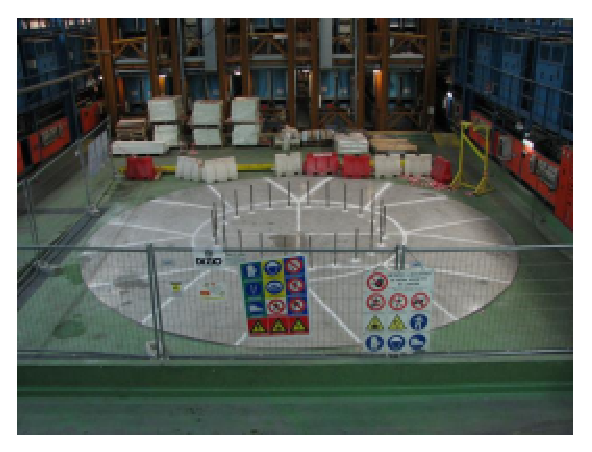
\includegraphics[height=0.23\textheight]{emptySite}}\hfil %
\subfloat[]{\label{fig:cryostat}
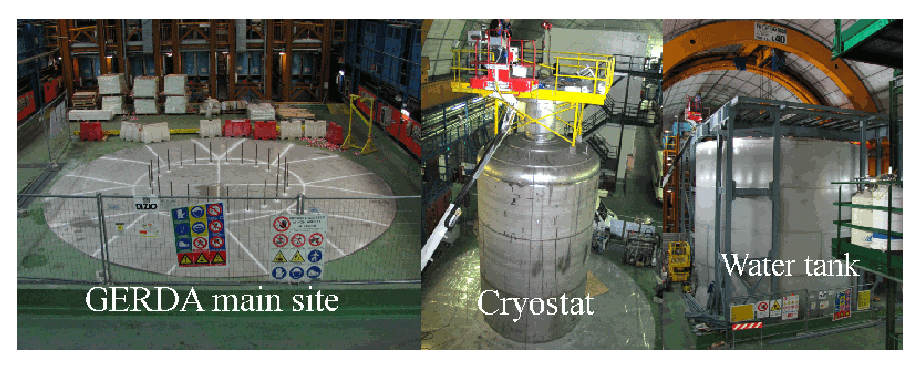
\includegraphics[height=0.23\textheight]{cryostat}}\hfil%
\subfloat[]{\label{fig:waterTank}
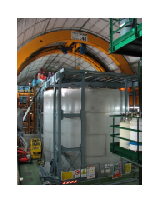
\includegraphics[height=0.23\textheight]{waterTank}}%
\caption{Construction of cryostat and water tank at the GERDA main
site: (a) empty GERDA main site, (b) cryostat and (c) water tank and
some infrastructure around it.}
\label{fig:cryo}
\end{figure}

\subsection{Clean room and lock system}
\label{sec:gerda:stat2}
Figure~\ref{fig:waterTank} shows the first parts of the superstructure
around the water tank, on top of which the clean room and lock will be
built. The clean room is under construction. The design of the lock
structure is almost finished. The lock will be pre-installed at the
Max-Planck-Institut f\"ur Physik in Munich and then transported to the
LNGS in 2009. A provisional lock system is in production. It will be
used before the complete lock system is ready, so that the
commissioning of GERDA can start in spring 2009.

\subsection{Phase I and II detectors}
\label{sec:gerda:stat3}
In total 17.9~kg of enriched and 15~kg of non-enriched high-purity
p-type germanium detectors from IGEX \cite{Aal02}, HdM \cite{Hei04}
and the Genius Test Facility (GTF) \cite{Kla02} will be operated in
Phase I of GERDA. The tests of these p-type detectors operated in
cryogenic liquids are practically completed.

A total of 37.5~kg of enriched germanium was procured for GERDA Phase
II detectors. It has an enrichment level of about 90\% and is stored
in the HADES facility in the form of GeO$_{2}$. The purification tests
with depleted germanium have shown that the yield for 6N material is
about 90\%, and the exposure time above ground will not exceed $2 \sim
3$ days. The resulting 6N material will be transformed into crystals
by the Institut f\"ur Kristallz\"uchtung (IKZ) in Berlin. Crystals
with a concentration of impurities down to $10^{11}$ per cm$^{3}$ have
been pulled at IKZ, see Fig.~\ref{fig:pulling}. The \u{C}zochralski
puller was already refurbished to produce larger crystals.
\begin{figure}[tbhp]
\centering
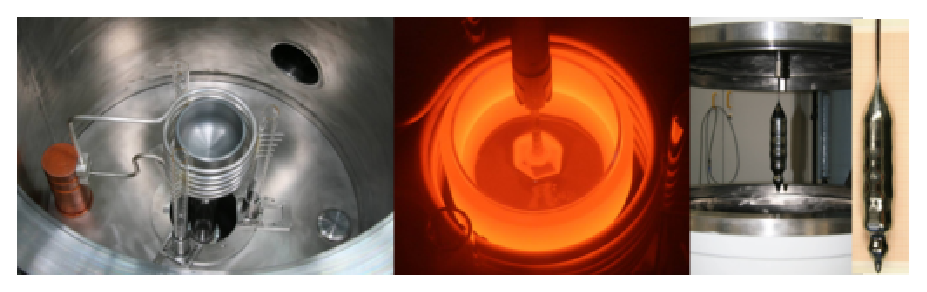
\includegraphics[width=\textwidth]{crystalPulling}
\caption{Pulling crystal in \u{C}zochralski puller (from left to
right): a \u{C}zochralski puller, growing crystal, cooled-off crystal
in open puller and a close-up of crystal.}
\label{fig:pulling}
\end{figure}

The first two prototype detectors for GERDA Phase~II were developed
and produced in close collaboration with the manufacturer
Canberra-France. They are called Siegfried I and Siegfried II. The
Siegfried series are $n$-type true coaxial cylindrical crystals made
of natural germanium with a height of 70~mm and a diameter of 75~mm
with a 10~mm hole in the center. The active volume is 302~cm$^{3}$,
the total mass is 1.6~kg. They are 18-fold segmented with a 6-fold
segmentation in the azimuthal angle $\phi$ and a 3-fold segmentation
in the height $z$. The segmentation scheme and the detector coordinate
system are depicted in Fig.~\ref{fig:ger:segm} where a scheme of the
cabling (left) and the segment numbering (right) are shown. The
segments are read out using a Kapton flexible printed-circuit-board
(FPCB) with snap-contacts \cite{Sie07}. Pictures of the two detectors
together with the contact cables are shown in
Fig.~\ref{fig:ger:sies}. The detector specifications as provided by
Canberra-France are summarized in Table~\ref{tab:tt:detpar}.

\begin{figure}[tbhp]
\centering
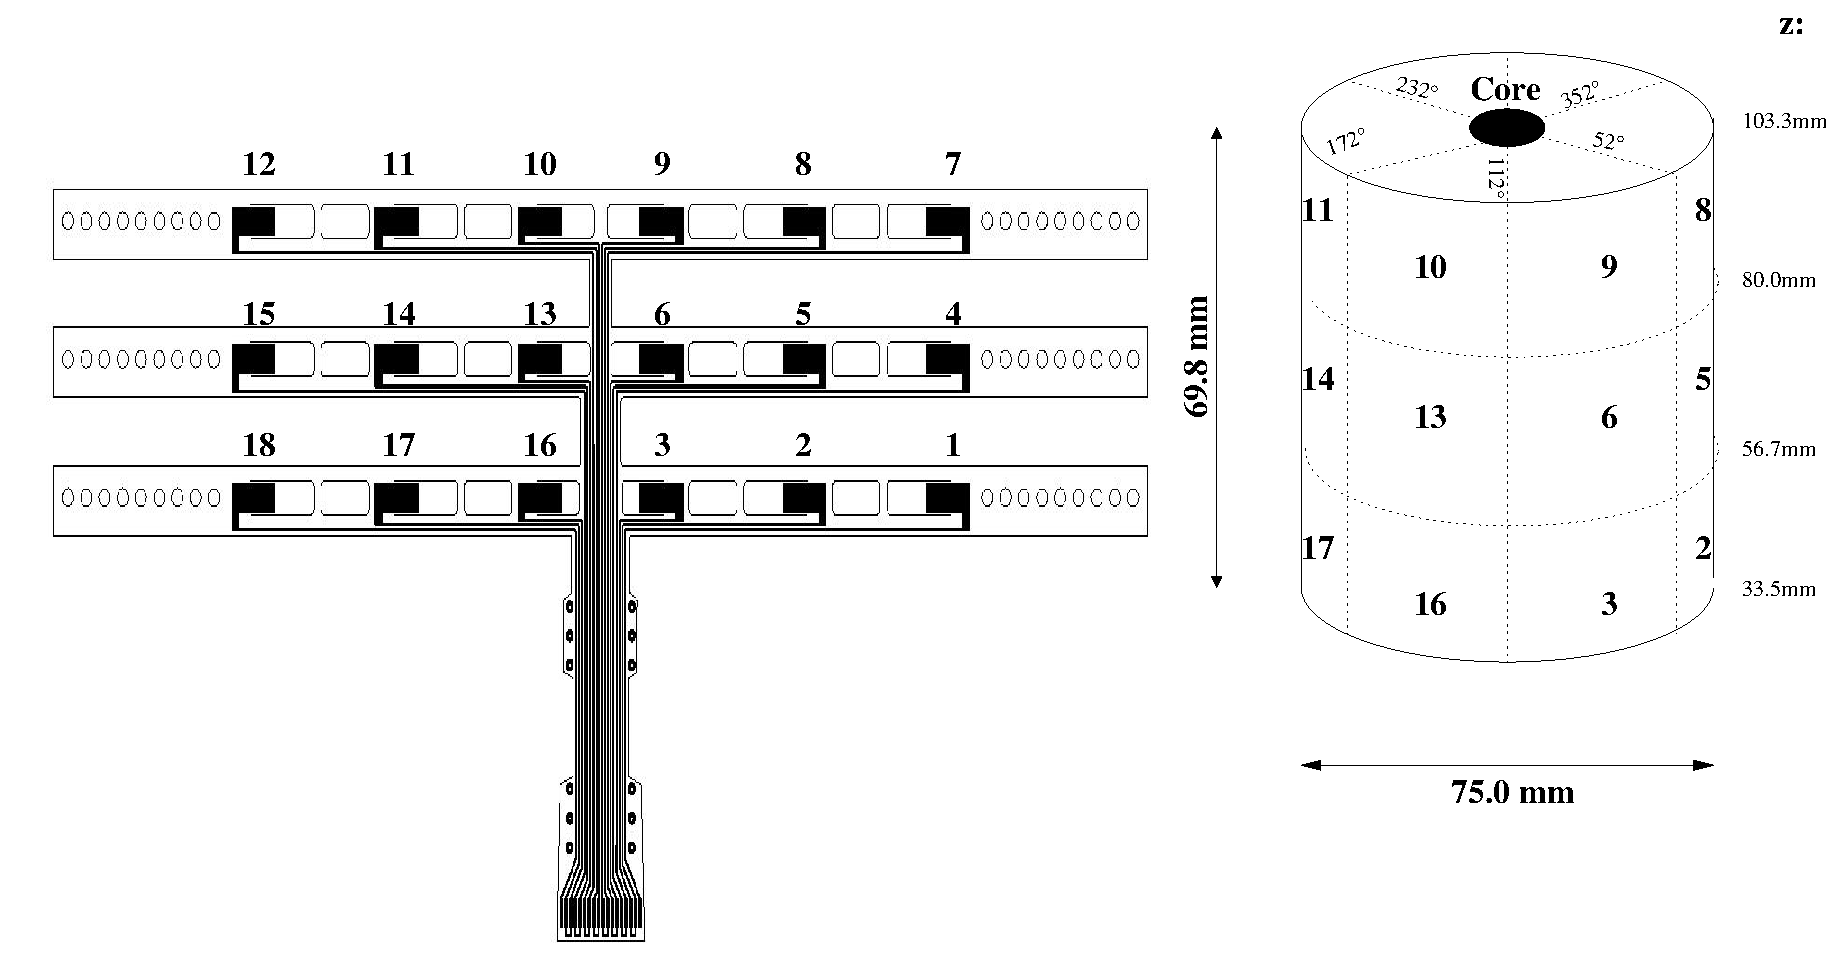
\includegraphics[width=0.9\textwidth]{segmentation_scheme}  
\caption{Schematic of cable (left) and segment numbering (right) of
the prototype detectors.}
\label{fig:ger:segm}
\end{figure}

\begin{figure}[tbhp]
\centering
\subfloat[]{\label{fig:ger:si}
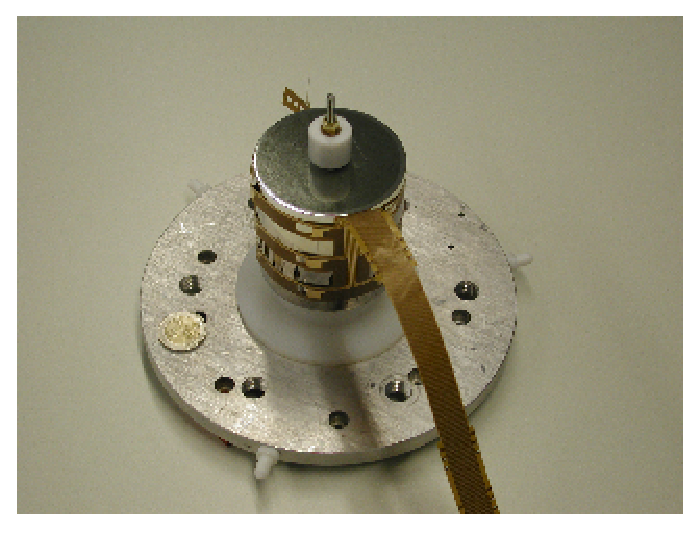
\includegraphics[height=0.23\textheight]{SiegfriedI}}\hfil %
\subfloat[]{\label{fig:ger:sii}
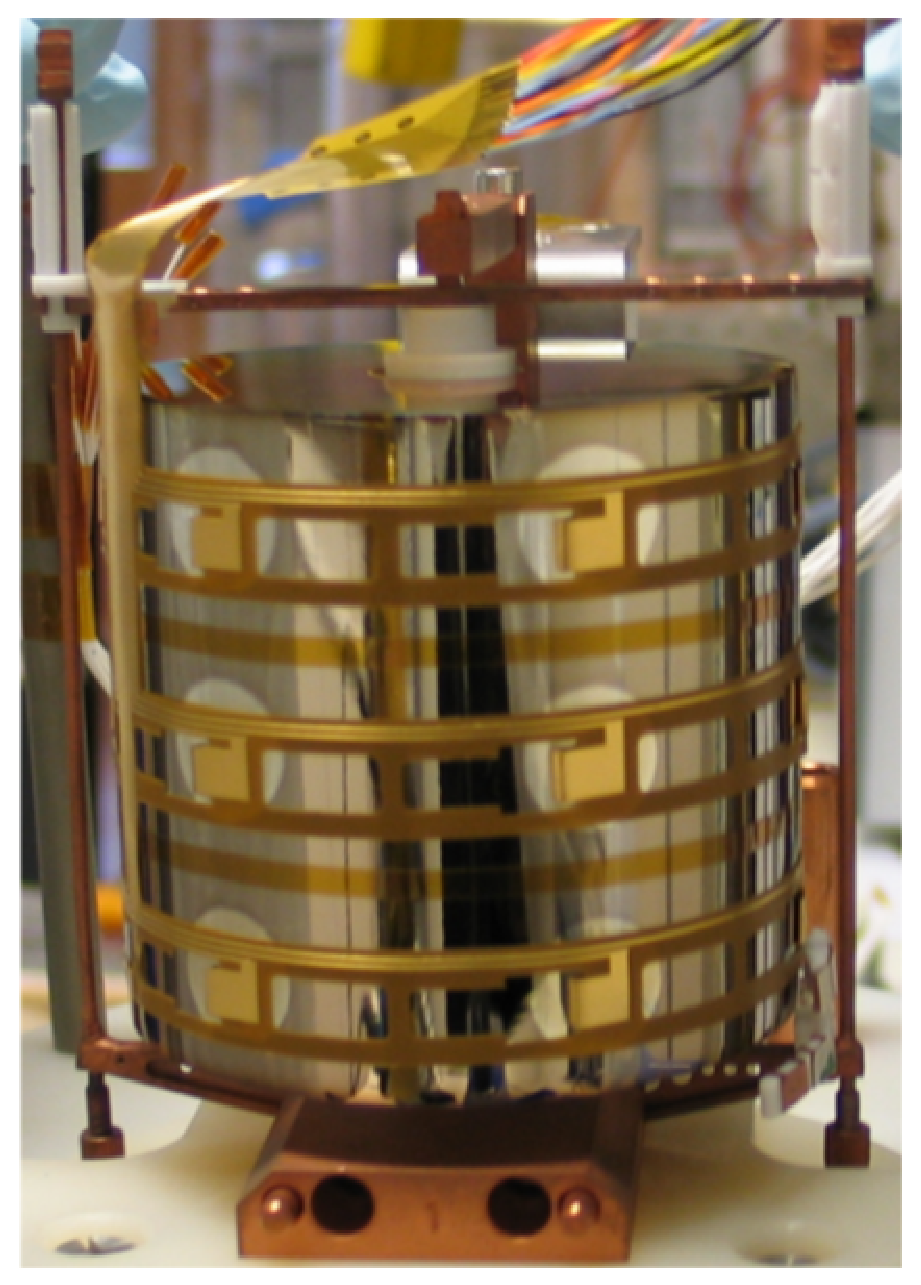
\includegraphics[height=0.23\textheight]{SiegfriedII}}%
\caption{Siegfried series of detectors with Kapton FPCB contact cables
around: (a)Siegfried I and (b) Siegfried II.}
\label{fig:ger:sies}
\end{figure}

\begin{table}[tbhp]
\centering
\caption{Detector specifications as provided by Canberra-France.}
\label{tab:tt:detpar}
\begin{tabular}{lll}\\\hline
Parameter & \emph{Siegfried} I  & \emph{Siegfried} II \\\hline
Outer diameter (mm)   & 75.0 & 75.2\\ 
Inner diameter (mm)   & 10 & 10 \\ 
impurity ($10^{10}$~cm$^{-3}$) & 
0.70(top), 1.35(bottom) & 0.35(top), 0.55(bottom) \\
Height (mm)           & 69.8 & 70.2 \\\hline 
Operating voltage (V) & +3000 & +2000 \\ 
FWHM at 122~keV (keV)  & 0.99 & 0.96 \\ 
FWHM at 1333~keV (keV) & 1.99 & 2.11 \\ \hline 
\end{tabular}
\end{table}

Siegfried I was operated in a conventional cryostat and extensively
tested and characterized \cite{Sie07}. Siegfried II was operated in
liquid nitrogen for five months. The handling, operating and testing
of the prototype detectors and the physics analyses based on the data
from them are the main topics of this thesis and will be discussed in
detail in the following chapters.

\section{Sensitivity}
\label{sec:gerda:sens}
A dedicated discussion of the sensitivity of GERDA can be found in
Ref.~\cite{Cal06}. Figure~\ref{fig:ger:llife} taken from
Ref.~\cite{Cal06} shows the expected 90\% probability lower limit on
the half-life of $0\nu\beta\beta$ decay versus the exposure under
different background conditions. Figure~\ref{fig:ger:lmass} shows the
expected 90\% probability upper limit on the effective Majorana
neutrino mass versus the exposure under different background
conditions.
\begin{figure}[tbhp]
\centering
\subfloat[]{\label{fig:ger:llife}
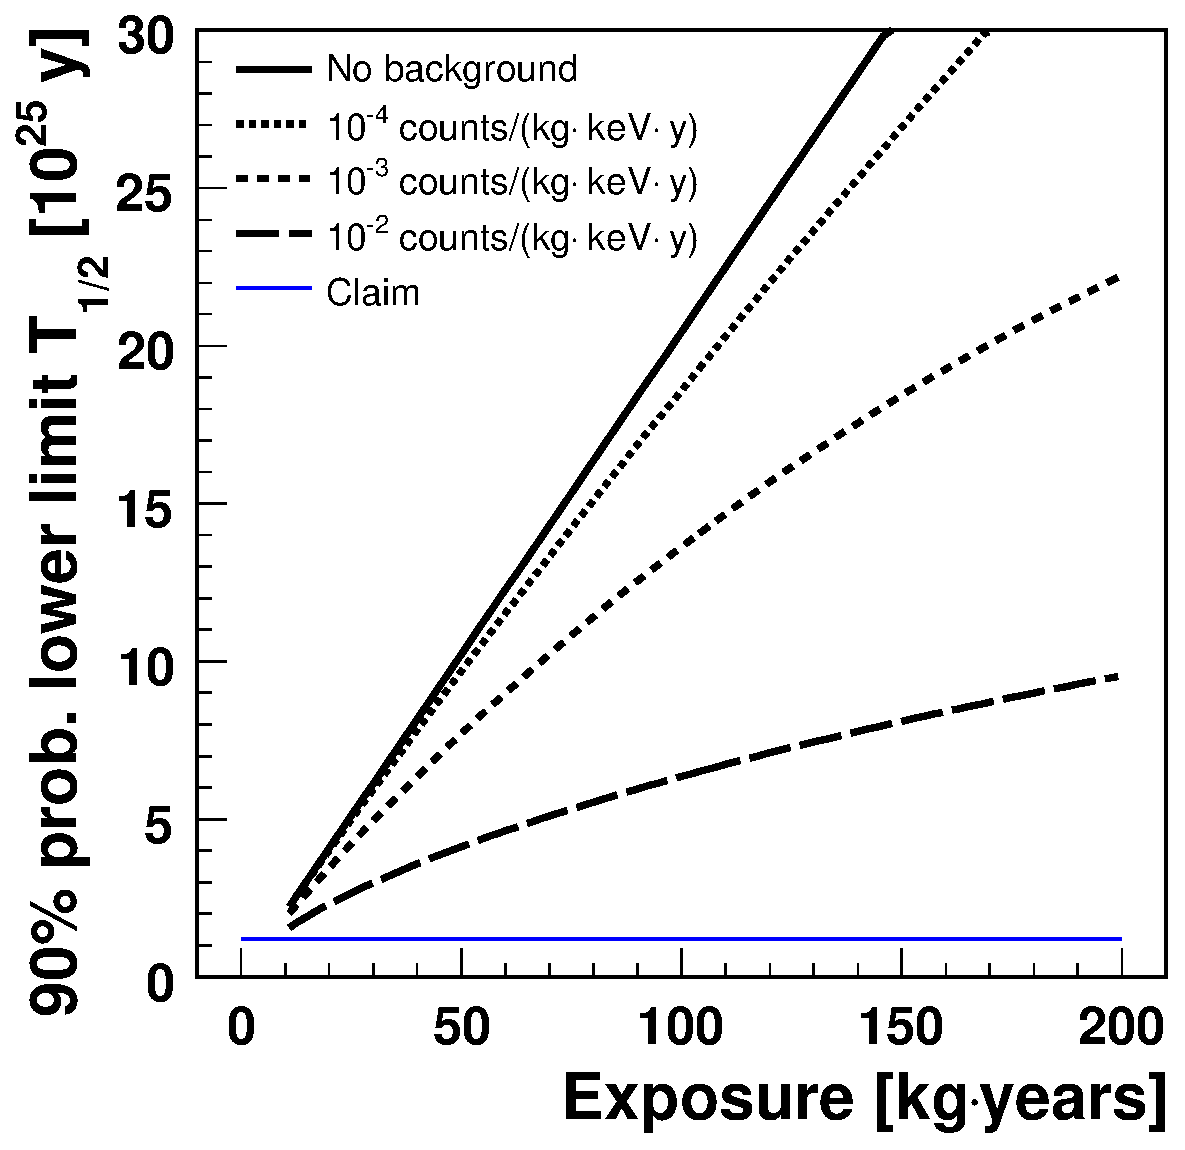
\includegraphics[width=0.4\textwidth]{limit_halflife}}\hfil%
\subfloat[]{\label{fig:ger:lmass}
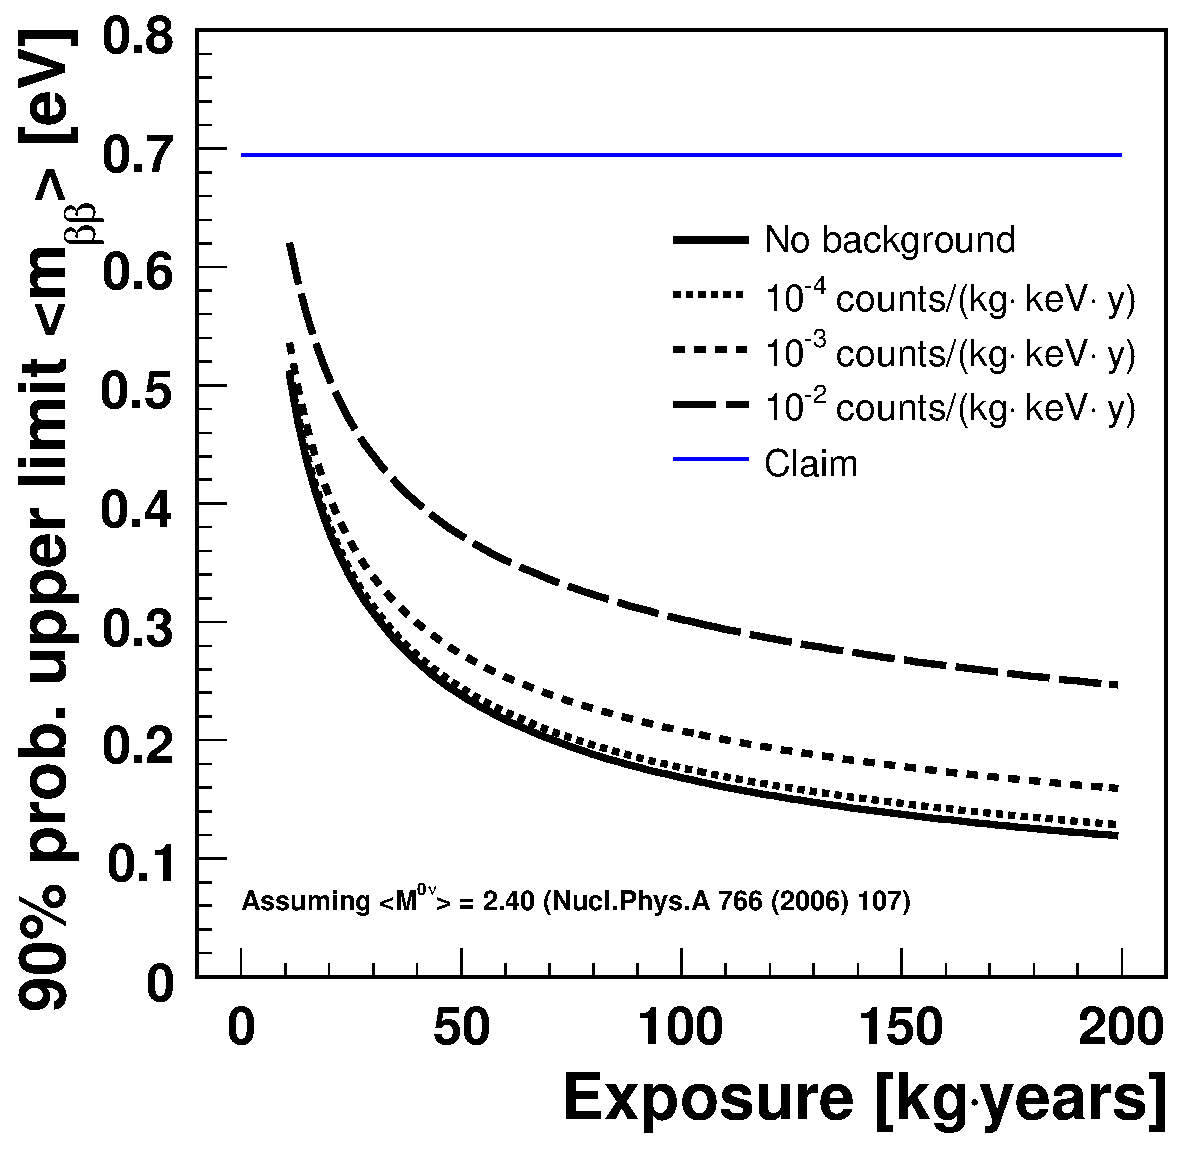
\includegraphics[width=0.4\textwidth]{limit_mass}}%
\caption{Sensitivity of GERDA: (a) the expected 90\% probability lower
limit on the half-life for $0\nu\beta\beta$ decay and (b) the
expected 90\% probability upper limit on the effective Majorana
neutrino mass versus the exposure under different background
conditions. Also shown is the half-life and the effective
Majorana neutrino mass for the claimed observation by
H. V. Klapdor-Kleingrothaus \textit{et al.} \cite{Hei04}. All mass
values are determined from the half-life using the matrix elements
reported in Ref.~\cite{Rod07}.}
\label{fig:gerda:limit}
\end{figure}

For GERDA Phase I, assuming a background level of
$10^{-2}$~events/(kg$\cdot$keV$\cdot$year) and an exposure of
30~(kg$\cdot$year), an upper limit on $m_{\beta\beta}$ of 0.42~eV is
achievable. For Phase II, assuming a background level of
$10^{-3}$~events/(kg$\cdot$keV$\cdot$year) and an exposure of
100~(kg$\cdot$year), an upper limit on $m_{\beta\beta}$ of 0.2~eV is
achievable.

%%% Local Variables:
%%% mode:latex
%%% TeX-master: "thesis"
%%% End:
